In this chapter, the performance of both the simulation model and visual SLAM method are analyzed in a series of experiments.
In Section \ref{sec:simulation_results}, the USARSim simulation model is validated.
I like to thank Carsten van Weelden for these experiments.
He flew a set of maneuvers with the actual AR.Drone and simulated AR.Drone. The differences between the maneuvers are studied in detail.
In Section \ref{sec:results-position-accuracy}, the accuracy of the estimated position is evaluated.
A set of 8-shapes is flown with the AR.Drone and the estimated positions are compared against the groundtruth from a laser range finder.
In Section \ref{sec:results-pose-recovery}, the proposed pose recovery approach is benchmarked against other pose recovery approaches.
In Section \ref{sec:res-cam-resolution}, the influence of the camera resolution is investigated.
Finally, in Section \ref{sec:results-elevation-accuracy} the accurracy of the elevation map is evaluated in terms of elevation error and the error in the estimated size of objects.


	\section{Simulation model}
\label{sec:simulation_results}
To evaluate the USARSim simulation model,  
a set of maneuvers is flown with the actual AR.Drone and
simulated AR.Drone. The differences between the maneuvers are studied in detail. To enable multiple repetitions of the same maneuver it is
described as a set of time points (milliseconds since initialization) each coupled to a movement command.
%We wrote wrappers for the AR.Drone programming interface and for USARSim interface which read these scripts and output a control
%signal, using the system clock to manage the timing independently from the game engine and the AR.Drone hardware.
Orientation, altitude and horizontal speed are recorded at a frequency of $200\hertz$ during the maneuvers. These are gathered through the AR.Drone's internal sensors and the onboard algorithms, which are
also used by the controller to operate the drone. The filtered output of the gyroscope is used
to estimate the orientation. The filtered output of the ultrasound distance sensor is used to estimate
the altitude. The onboard visual odometry algorithm is used to estimate the horizontal (linear
and lateral) speeds. The simulator has equivalent sensors. In addition, simulation can provide ground-truth data. 
Also for the real maneuvers an attempt was made to generate ground truth via an external reference system; the movements were recorded with a synchronized video system consisting of four firewire cameras, capturing images at 20 frames per second at a resolution of $1024 \times 768$ pixels. The position of the AR.Drone 
in each frame has been annotated by hand. 
%However, since the processing of the captured data is not yet complete, results from these trials are not presented in this paper.
%reference?!

Corresponding to NIST guidelines \cite{Jacoff2010STM}
a set of experiments of increasing complexity was performed. For the AR.Drone
four different experiments were designed.
The first experiment is a simple hover, in which the drone tries to maintain its position (both horizontal and vertical). The second experiment is linear movement, where the drone actuates a single movement command. The third experiment is a small horizontal square. The last experiment is a small vertical square.

\subsubsection{Hovering}

Quadrotors have hovering abilities just like a helicopter. The stability in maintaining a hover depends
on environmental factors (wind, underground, aerodynamic interactions) and control software.
%In \cite{Michael2010ra} a
%horizontal positioning error of no more than $2\small{cm}$ and a vertical error of less than $0.6\small{cm}$ are reported for
%a tightly optimized stiff controller. In practice, softer controllers are used which are more robust and can
%recover from larger disturbances. In \cite{How2008} a horizontal and vertical positioning error of no more than $10\small{cm}$ are %reported. 
If no noise model is explicitly added, the USARSim model performs a perfect hover; when no control signal is given the
horizontal speeds are zero and the altitude stays exactly the same.

For the AR.Drone, this is a good zero-order model. One of the commercial features of the AR.Drone is its ease of operation. As part of this feature it
maintains a stable hover when no other commands are given, which is accomplished by a visual feedback loop.
%The hover is quite robust and in impromptu
%ad-hoc tests was able to recover from major attitude disturbances up to $\sim45^o$. However, in this section we
%are concerned with the hovering behavior with minor disturbances. 
So, the hovering experiment is performed  
indoors
with an underground chosen to have enough texture for the onboard visual odometry estimation algorithm.

As experiment the AR.Drone maintained a hover for $35$ seconds. This experiment was repeated $10$ times,
collecting $60.000$ movement samples for a total of $350$ seconds. Over all samples the mean absolute error in horizontal
velocity (the Euclidean norm of the velocity vector) was $0.0422\small{m/s}$ with a sample variance of $0.0012\small{m^2/s^2}$. The distribution of the linear and lateral velocity components was obtained from the samples.

From the velocity logs the position of the AR.Drone during the $35$-second 
flight was calculated. 
%Figure \ref{fig:scatterplot} shows a scatterplot of positions over all flights.
The mean absolute error of the horizontal position was $0.0707\small{m}$ with a sample variance of $0.0012\small{m^2}$.

\begin{comment} % to save some space
\begin{figure}[htb]
\centering
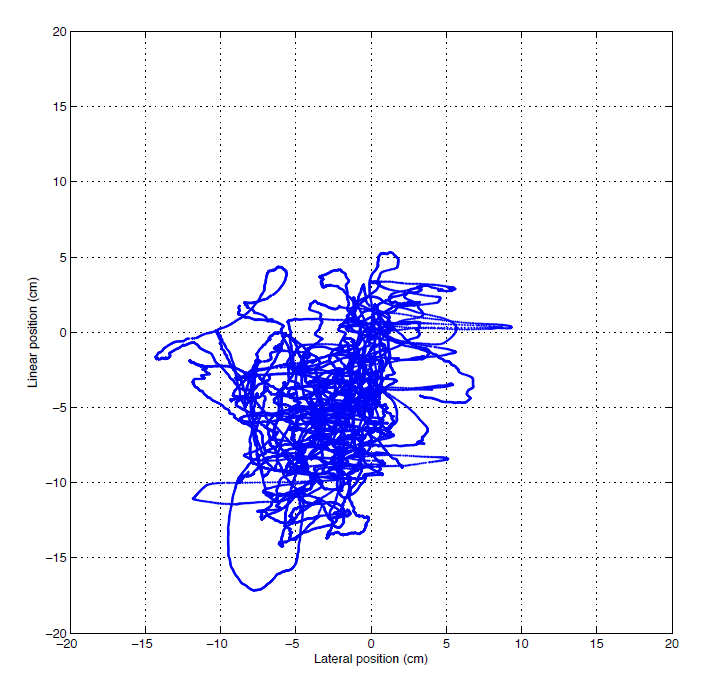
\includegraphics[width=8cm]{images/HoverScatterPlot.png}
\caption{Scatter plot of the horizontal position aggregated over all hover flights.}
\label{fig:scatterplot}
\end{figure}
\end{comment}

\subsubsection{Horizontal movement}

In this experiment the AR.Drone is flown in a straight line. It is given a control pulse (i.e., pitch) with a constant signal
for 5 different time periods: $0.1\small{s}$, $1\small{s}$, $2\small{s}$, $3\small{s}$, and $5\small{s}$. Each pulse is followed by a null signal for enough time for the AR.Drone to make a full stop and a negative pulse of the same magnitude for the same period,
resulting in a back and forth movement. In Figure \ref{fig:RealResponse}
 the red line shows the control signal, the blue line the response (i.e., velocity) of the AR.Drone. The experiment was repeated for 5 different speeds.
The control signal $s$ specifies the pitch of the AR.Drone as a factor (between $0$ and $1$) of the maximum absolute tilt $\theta_{max}$, which was set to the default value\footnote{ARDrone firmware (1.3.3)}. % iPhone uses 12deg
The trials were performed with the
values of $0.05$, $0.10$, $0.15$, $0.20$, $0.25$ for the control signal $s$.

\begin{figure}[htb]
\centering
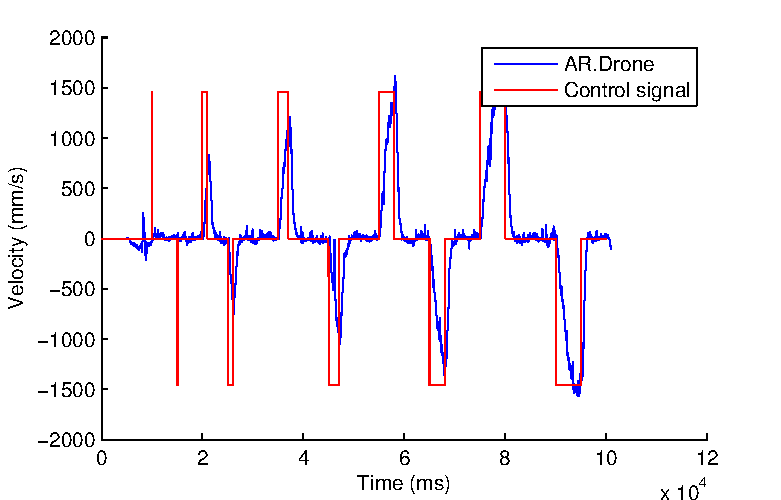
\includegraphics[width=11cm]{images/Dr7Ov-eps-converted-to.pdf}
\caption{Velocity of the real AR.Drone (blue) on a number of control pulses (red) with a pitch of $s=0.15 \times \theta_{max}$ .}
\label{fig:RealResponse}
\end{figure}

Robots in USARSim are controlled with a standardized interface, which uses SI units. A robot in USARSim expects a DRIVE command with a speed in $m/s$ and not the AR.Drone native signal $s$. 
Thus in order to 
fly comparable trials 
the relation between the AR.Drone's angle of attack $\alpha$ and the corresponding velocity $v$ has to be investigated.
When flying straight forward in no-wind conditions, the angle of attack $\alpha$ is equivalent with the pitch $\theta$.
In order to do this the samples from the logs where the AR.Drone has achieved maximum
velocity have to be selected. Closer inspection of the velocity logs show that in each trial there is still constant increase of velocity for the first three pulses. For the last two pulses there is obvious plateauing, which indicates that the last two seconds of the five-second pulses is a good indication for the maximum velocity. Therefore the velocity at those
last two seconds was used to compute mean absolute speeds $\bar{v}$, which are combined with the mean absolute
pitch $\bar{\theta}$ as measured by the MEMS gyroscope. The estimates for $\bar{v}$ and pitch $\bar{\theta}$ are presented in Table~\ref{tab:angle_of_attack} together with their standard deviation. 
% Looking at the values for the pitch we see that these differ from the expected angles listed above.
Extrapolating the mean pitch $\bar{\theta}\simeq7.5^o$ at 
control value $s=0.25$ to the maximum control signal gives an indication of
the AR.Drone's maximum pitch $\theta_{max}\simeq30^o$ value. For typical usage, the angle of attack never exceeds $12^o$ degrees.

\begin{table}[htb]    \centering
    \begin{tabular}
        { | l | l  l  l  l  l | }
        \hline 
          &  \multicolumn{5}{| l |}{Control signal $s$} \\
          & 0.05 & 0.10 & 0.15 & 0.20 & 0.25 \\    
        \hline
        $\bar{v}$ (m/s) & 0.4044 & 0.6284 & 1.4427 & 1.7587 & 2.2094 \\
        $\sigma_v$ (m/s) & 0.096 & 0.226 & 0.070 & 0.126 & 0.165 \\
        \hline
        $\bar{\theta}$ (deg) & 1.4654 & 2.9025 & 4.1227 & 5.7457 & 7.4496 \\
        $\sigma_\theta$ (deg) & 0.455 & 0.593 & 0.482 & 0.552 & 0.921 \\
        \hline
    \end{tabular}    \caption{Averaged velocity $\bar{v}$ measured at the end of a 5 seconds pulse of the control signal $s$, including the corresponding pitch $\bar{\theta}$ as measured by the gyroscope.}
    \label{tab:angle_of_attack}
\end{table}

\begin{comment}
\begin{table}[htb]    \centering
    \begin{tabular} 
        { | l | l | l | l | l | l | }
        \hline 
          &  \multicolumn{5}{|l|}{Control signal $s$} \\
          & 0.05 & 0.10 & 0.15 & 0.20 & 0.25 \\
        \hline
        $\bar{v}$ (m/s) & 0.4044 & 0.6284 & 1.4427 & 1.7587 & 2.2094 \\
        $\sigma_v$ (m/s) & 0.096 & 0.226 & 0.070 & 0.126 & 0.165 \\
        \hline
        $\bar{\theta}$ (deg) & 1.4654 & 2.9025 & 4.1227 & 5.7457 & 7.4496 \\
        $\sigma_\theta$ (deg) & 0.455 & 0.593 & 0.482 & 0.552 & 0.921 \\
        \hline
    \end{tabular}    \caption{Averaged velocity $\bar{v}$ measured at the end of a 5 seconds pulse of the control signal $s$, including the corresponding pitch 
$\bar{\theta}$ as measured by the IMU.} 
    \label{tab:angle_of_attack}
\end{table}
\end{comment}

To convert the AR.Drone's control signal $s$ to USARSim commands $v$ a least-squares fit through the points of Table~\ref{tab:angle_of_attack} is made for the linear function
$v = c \cdot \theta$, which gives $c=0.2967$. 
Equation \ref{eq:conversion} gives the final conversion of a control signal $s$ to a velocity $v$ in $m/s$ given the
AR.Drone's maximum pitch $\theta_{max}$ in degrees.

\begin{equation}
v = 0.2967 \cdot s \cdot \theta_{max}
\label{eq:conversion}
\end{equation}

The USARSim model has a parameter $P_\theta$ for calculating the angle (radian) given the velocity, which
% we can calculate from the coefficient $c$ above by converting from degrees to radians. This gives the
% theoretical $P_\theta = \frac{1}{0.2967} \cdot \frac{\pi}{180} = 0.0588$. However, doing a least-squares fit on the angle given the velocity gives 
is the value $\hat{P}_\theta = 0.057$, as used in subsequent simulations.

The next experiment checks the acceleration of the real and simulated AR.Drone.
An estimate describes how quickly the AR.Drone's controller changes its pitch to match the commanded pitch and how well it can keep it.
Samples are selected from $100\small{ms}$ after the start
of the $2\small{s}$, $3\small{s}$ and $5\small{s}$ pulses till the commanded pitch has been reached.
This
corresponds to the time-span between which the AR.Drone has started to act on the change in the control
signal until it reaches the commanded pitch. The result is illustrated in Figure \ref{fig:ComparisonOfResponse}.

\begin{figure}[htb]
\centering
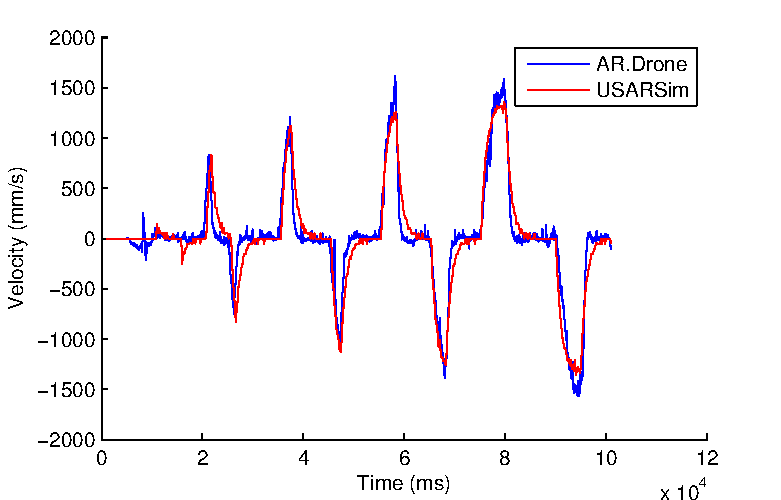
\includegraphics[width=11cm]{images/RYtdB-eps-converted-to.pdf}
\caption{Velocity of the real (blue) and simulated AR.Drone (red) on the same control pulses as shown in Figure~\ref{fig:RealResponse}.}

\label{fig:ComparisonOfResponse}
\end{figure}

As one can see, the acceleration shows for the real and simulated AR.Drone nearly the same slope. The deceleration of the simulated AR.Drone is slightly lower. In the real AR.Drone the feedback loop (based on the onboard visual odometry of the ground camera) actively decelerates the system. Overall, the dynamic behavior of the simulator closely resembles the dynamic behavior of the real system. Additionally, tests with more complex maneuvers (horizontal and vertical square) have been recorded, but unfortunately not analyzed in detail.




\section{Position accuracy}
\label{sec:results-position-accuracy}
An experiment has been carried out to evaluate the accuracy of the AR.Drone's estimated position.
This experiment is performed above a texture-rich floor (Section \ref{sec:exp1-texture-poor}), a texture-poor floor (Section \ref{sec:exp1-texture-poor}) and a floor that resembles the circumstances encountered during the IMAV competition.
The position can be estimated using different methods and the accuracy of all these methods are evaluated.
To ensure fair comparison of the different estimation methods, a flight was recorded (Section \ref{sec:proposed-framework}) and played back to generate the same input for all methods.

The first position estimation method integrates the AR.Drone's onboard velocity (AV) measurements to estimate the position (Section \ref{sec:pose_estimation}).
Recent versions of the AR.Drone firmware calculcate an estimated position onboard\footnote{Firmware 1.7.4}, which is used as second estimation method.
The third position estimation method uses the visual odometry method presented in this thesis (Section \ref{sec:visual-slam-visual-odemetry}).
The final estimation method uses the AR.Drone's onboard velocity (AV) for frequent position updates and the presented localization method (Section \ref{sec:localization}) to localize against the map that is constructed during flight.

The estimated position is compared against the groundtruth (real) position to calculcate the accuracy of the estimated position.
Much attention was paid to collect accurate groundtruth of the AR.Drone's position.
A high-end laser range finder (LRF)\footnote{Hokuyo UTM-30LX, \url{http://www.hokuyo-aut.jp/02sensor/07scanner/utm_30lx.html}} was used to determine the position of the AR.Drone.
The LRF measures distance to objects.
A window was placed on the measurements to filter out measurements that originate from the environment.
All remaining distance measurements are assumed to originate from the AR.Drone.
The mean position of the filtered distance measurements is used as center position of the AR.Drone.
Futhermore, a white cylinder with a diameter of 9\begin{small}cm\end{small} and a height of 37\begin{small}cm\end{small} was added on top of the AR.Drone to improve its visability for the LRF.

\begin{figure}[htb]
\centering
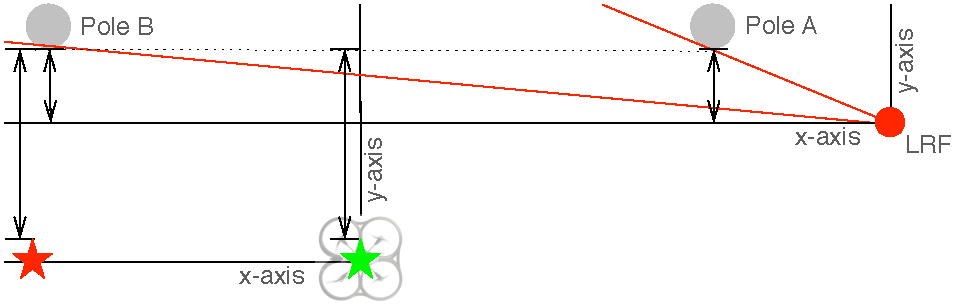
\includegraphics[width=13cm]{images/exp1-floorplan-align.pdf}
\caption{The alignment of the laser range finder and the AR.Drone. The laser range finder (LRF) is aligned against two poles. The takeoff position is marked with a green star. The red star indicates the marked heading direction of the AR.Drone. A laser pointer is used to align the heading direction of the AR.Drone to the marker position.}
\label{fig:exp1-floorplan-align}
\end{figure}

The LRF measures the AR.Drone's position in its own reference frame.
Therefore, the AR.Drone's reference frame has to be accurately aligned with the LRF's reference frame.
This is achieved by rotating the AR.Drone before takeoff, such that it points in exactly the same direction as the LRF.
The following method was used to align the LRF and the AR.Drone (Figure \ref{fig:exp1-floorplan-align}).
First, the LRF is aligned against two poles in the environment.
The LRF is rotated until both poles obtained an equal y-distance in the LRF's reference frame.
Now, the LRF's x-axis is parallel to the poles.
Next, the AR.Drone's takeoff position and orientation are determined.
The takeoff position is marked on the floor (green star).
Another position is marked (red star) to indicate the desired heading direction of the AR.Drone.
Both marked positions are parallel to the LRF's x-axis and the two poles.
Finally, a laser pointer is used to align the heading direction of the AR.Drone to the marked position.





\subsection{Texture-rich floor}
\label{sec:exp1-texture-rich}
The first experiment was performed above a texture-rich floor (Figure \ref{fig:exp1-floor}), to benchmark the methods in preferable circumstances.
Magazines were spraid out on the floor to provide sufficient texture for the computer vision algorithms.
The AR.Drone flew three 8-shapes above the magazines.
An 8-shape was chosen to capture an intermediate loop.

\begin{figure}[htb!]
\centering
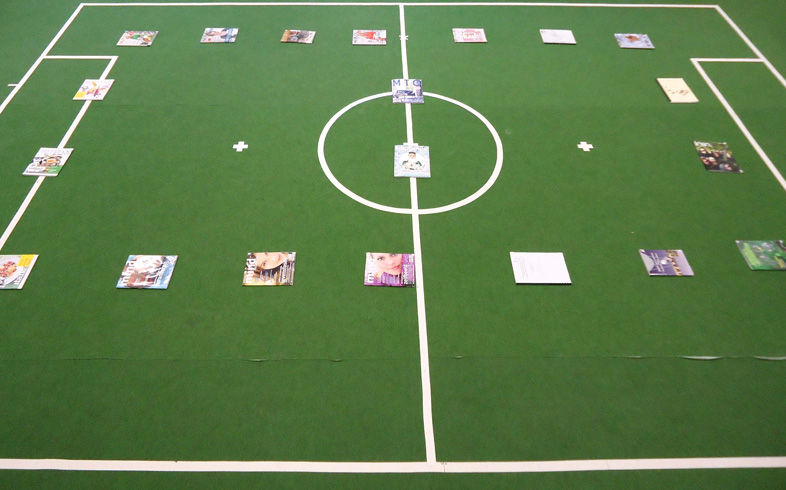
\includegraphics[width=8cm]{images/exp1-floor.jpg}
\caption{Photo of the texture-rich floor used for the first experiment. Magazine are spraid out on the floor to provide sufficient texture. The dimensions of the 8-shape are approximately $5\small{m} \times 2.5\small{m}$.}
\label{fig:exp1-floor}
\end{figure}

\begin{table}[htb!]
    \centering
    \begin{tabular}
        { | l | l | l | } 
	\hline
	Method & Mean absolute error (\small{mm}) & Mean relative error (percentage of trajectory length) \\
        \hline
	AP (onboard position) & 476 & 0.714\% \\
        AV (onboard velocity) & 477 & 0.715\% \\
	AV + localization & 260 & 0.390\% \\
	VO (visual odometry) & 552 & 0.828\% \\
	VO + localization & 324 & 0.486\% \\
	\hline
    \end{tabular}
    \caption{Errors made by the position estimation methods when flying above a texture-rich floor.}
    \label{tab:res_mapping}
\end{table}

\begin{figure}[htb!]
\centering
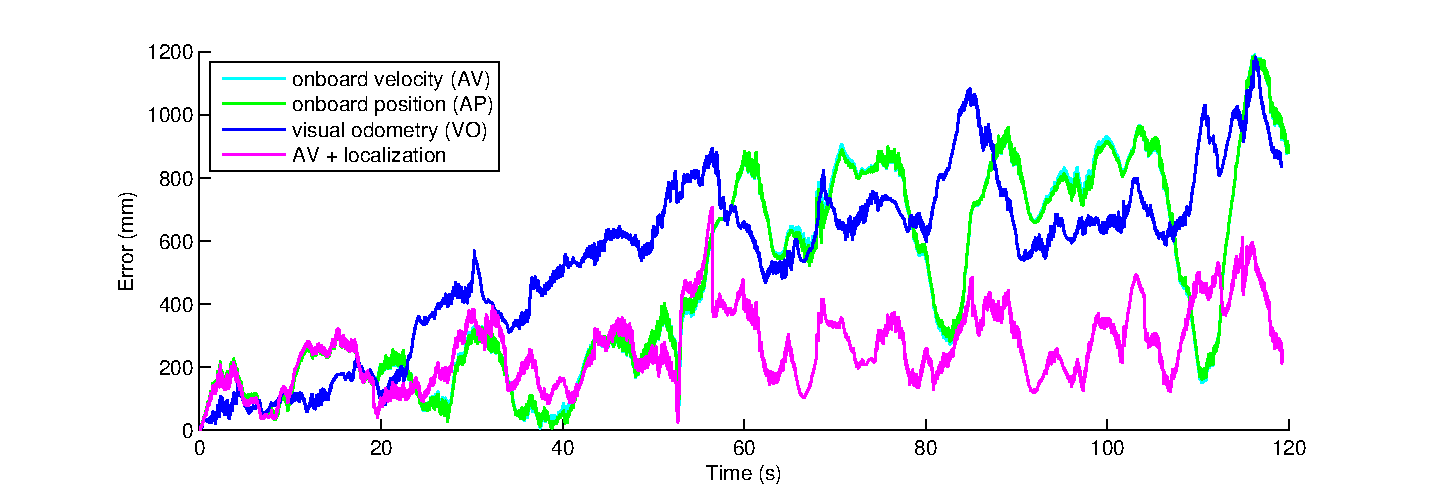
\includegraphics[width=\linewidth]{images/exp1-run13-error.eps}
\caption{Errors between the estimated positions and the groundtruth.}
\label{fig:exp1-texture-error}
\end{figure}

\begin{figure}[htb!]
\centering
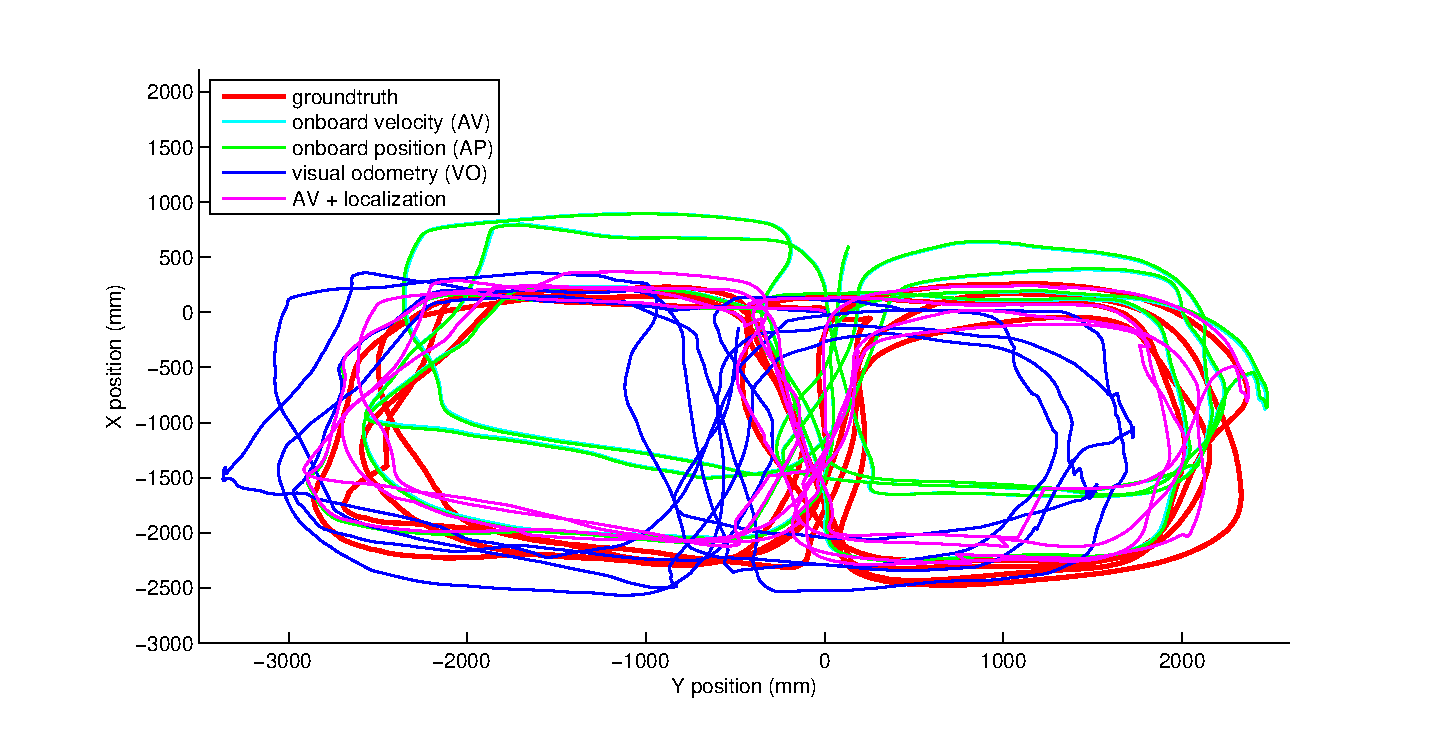
\includegraphics[width=\linewidth,trim=2cm 1.5cm 2cm 2cm]{images/exp1-run13-path.eps}
\caption{Estimated trajectories of the different position estimation methods. The AR.Drone flew three 8-shapes above a texture-rich floor.}
\label{fig:exp1-texture-path}
\end{figure}

\begin{figure}[htb!]
\centering
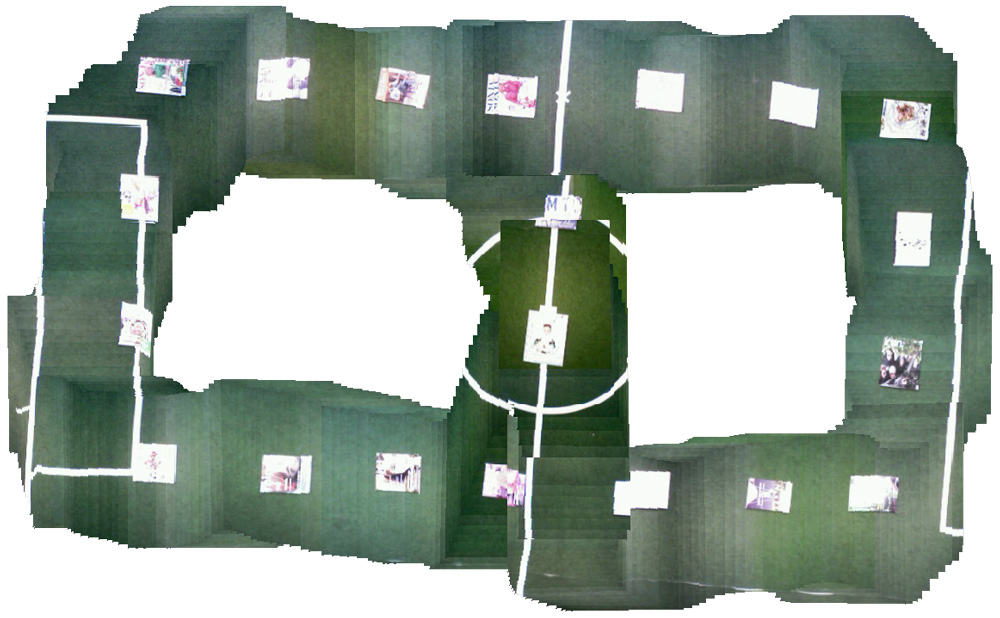
\includegraphics[width=0.75\linewidth]{images/exp1-run13-map.jpg}
\caption{Visual map created by the visual mapping method (Section \ref{sec:texture_map}). The map is constructed during the first 8-shape. The position estimates are based on the onboard velocity (AV) and the visual localization method (Section \ref{sec:localization}).}
\label{fig:exp1-texture-map}
\end{figure}

The results of this experiment can be found in Table \ref{tab:res_mapping} and Figures \ref{fig:exp1-texture-error} (errors), \ref{fig:exp1-texture-path} (trajectories) and \ref{fig:exp1-texture-map} (visual map).
For the encountered circumstances, all methods are able to estimate the position quite accurately.
Both the onboard velocity (AV) method and the onboard position (AP) method produce exactly the same trajectory and error, which implies the onboard position estimate (AP) is based on the velocity that is estimated by the AR.Drone.
Therefore, the onboard position estimate is omitted from all plots.

The onboard velocity (AV) slightly outperforms the visual odometry (VO) method presented in Section \ref{sec:visual-slam-visual-odemetry}.
An explanation could be that the AR.Drone features an additional optical flow algorithm that is used when the appearance-based method is performing badly.
From Figure \ref{fig:exp1-texture-path} can be seen that the onboard velocity (AV) method has the largest error in the x-direction.
Around $54\begin{small}s\end{small}$ the error is increasing rapidly.
Analysis of the dataset pointed out that a small part of a magazine and a large part of a white line were in range of the camera.
This resulted in a velocity thas was estimated in the wrong direction along the white line, which can be recognized by the small green loop on the right side of Figure \ref{fig:exp1-texture-path}.

The visual odometry (VO) method has the largest error in the y-direction.
Around $80\begin{small}s\end{small}$ the error is increasing rapidly.
Analysis of the dataset pointed out that the magazines were out of the camera's range. During this period the velocities could not be updated.

A combination of the onboard velocity (AV) with localization against the map outperforms all other methods.
With localization against the map, the error is reduced significantly.
%The map is constructed during the first 8-shape (first $40\begin{small}s\end{small}$).
From Figure \ref{fig:exp1-texture-error} can be seen that the maximum error is not exceeding the error made during the first 8-shape.
The repetitive error pattern suggests that the error of the estimated position largely depends on the quality (accuracy) of the map, if localization can be performed regularly.
%Around $85\begin{small}s\end{small}$ the error increases rapidly. This error is caused by a false match %against the map. However, future localizations correct this mistake.

The visual map (Figure \ref{fig:exp1-texture-map}) shows that the AR.Drone's onboard white balancing is reducing the contrast of the magazines, which affects the performance of the feature detector.
This is a source of error for the visual odometry (VO) algorithm.
Futhermore, errors in the ultrasound and IMU measurements are other sources that result in errors in the estimated velocities.

% 66674 mm






\subsection{Texture-poor floor}
\label{sec:exp1-texture-poor}
The experiment is repeated above a floor with low texture, to benchmark the methods in difficult circumstances.
Therefore, all magazines (Figure \ref{fig:exp1-floor}) are removed, resulting in a green floor with few white lines.
The AR.Drone flew a single 8-shape.


% 19616
\begin{table}[htb!]
    \centering
    \begin{tabular}
        { | l | l | l | } 
	\hline
	Method & Mean absolute error (\small{mm}) & Mean relative error (percentage of trajectory length) \\
        \hline
	AP (onboard position) & 1294 & 6.597\% \\
        AV (onboard velocity) & 1292 & 6.586\% \\
	VO (visual odometry) & 1126 & 5.740\% \\
	\hline
    \end{tabular}
    \caption{Errors made by the position estimation methods when flying above a texture-poor floor.}
    \label{tab:res_mapping-poor}
\end{table}

\begin{figure}[htb!]
\centering
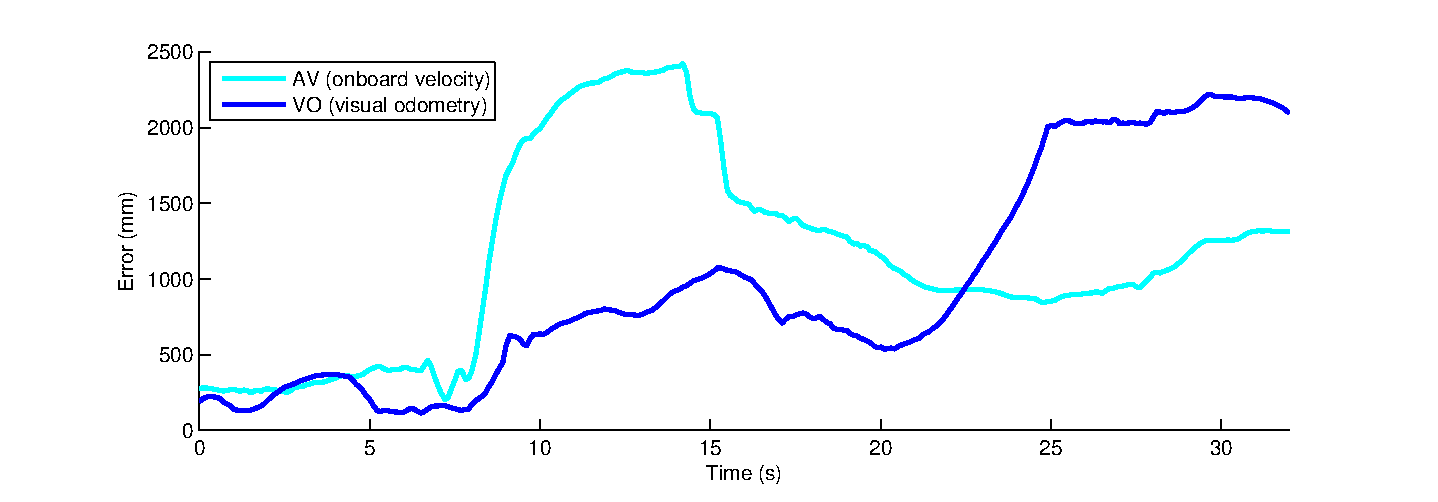
\includegraphics[width=\linewidth]{images/exp1-run2-error.eps}
\caption{Errors made by the position estimation methods when flying above a texture-poor floor.}
\label{fig:exp1-notexture-error}
\end{figure}

\begin{figure}[htb!]
\centering
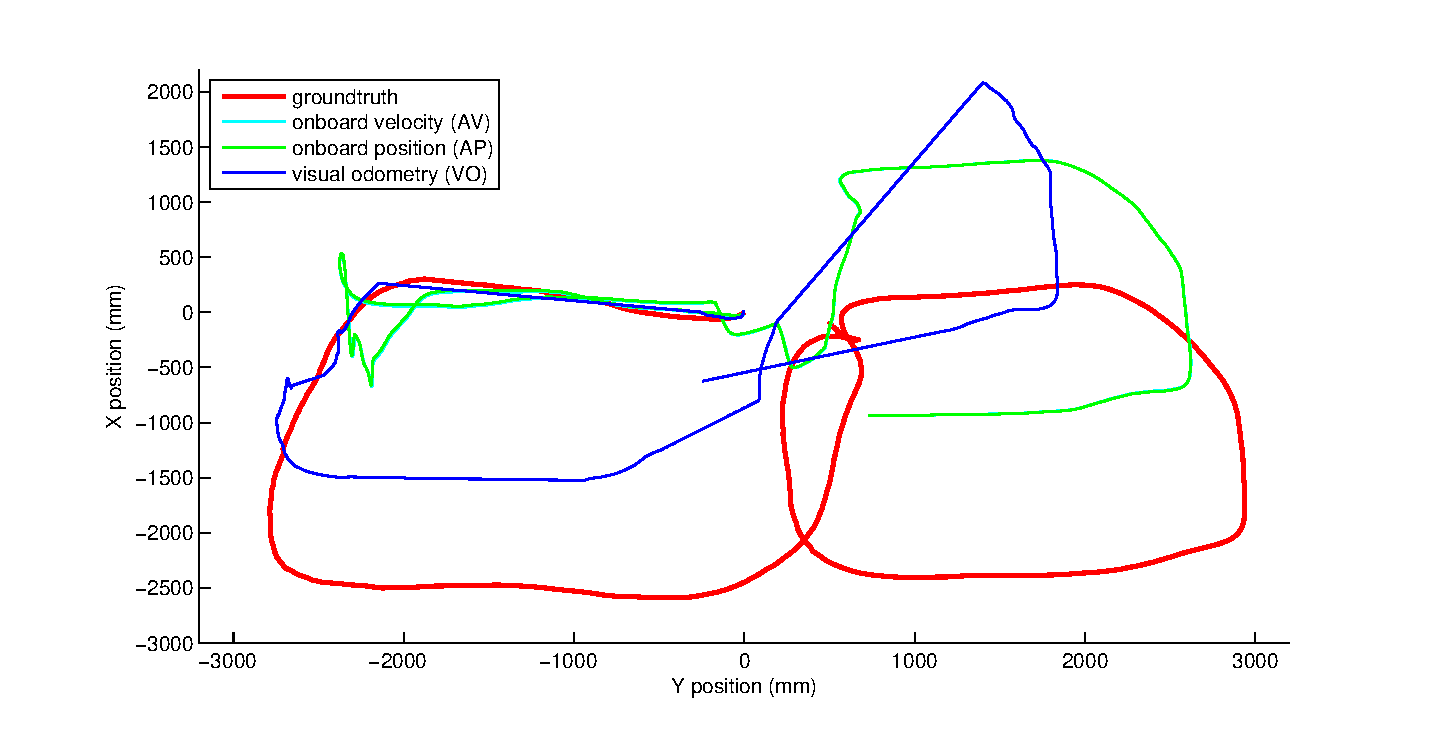
\includegraphics[width=\linewidth,trim=2cm 1.5cm 2cm 1cm]{images/exp1-run2-path.eps}
\caption{Estimated trajectories of the different position estimation methods. The AR.Drone flew three 8-shapes above a texture-poor floor.}
\label{fig:exp1-notexture-path}
\end{figure}

\begin{figure}[htb!]
\centering
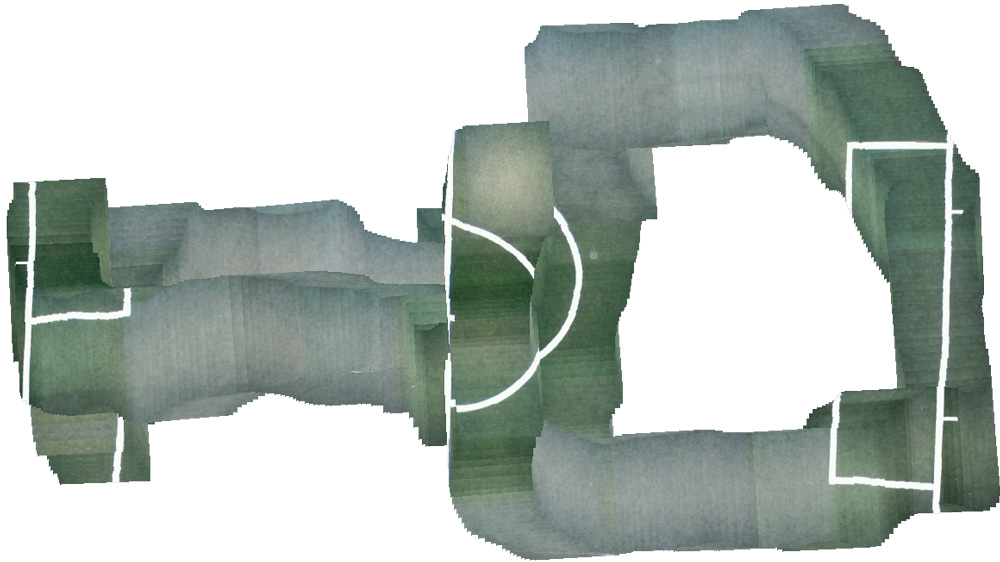
\includegraphics[width=0.75\linewidth]{images/exp1-run2-map.jpg}
\caption{Visual map created by the visual mapping method (Section \ref{sec:texture_map}). The position estimates are based on the onboard velocity (AV).}
\label{fig:exp1-notexture-map}
\end{figure}


The results of this experiment can be found in Table \ref{tab:res_mapping-poor} and Figures \ref{fig:exp1-notexture-error} (errors), \ref{fig:exp1-notexture-path} (trajectories) and \ref{fig:exp1-notexture-map} (visual map).
For the encountered circumstances, all methods are unable to estimate the position accurately.
Again, both the onboard velocity (AV) method and the onboard position (AP) method produce exactly the same trajectory.
Localization was not possible and therefore omitted from the plots.

The visual odometry (VO) method slightly outperforms the onboard velocity (AV) method.
One would expect that the AR.Drone's additional optical flow method outperforms appearance-based methods.
From Figure \ref{fig:exp1-notexture-path} can be seen that the onboard velocity (AV) method fails to correctly deal with the lines on the floor.
The onboard velocity (AV) methods measures a velocity in the wrong direction along the lines, resulting in a large error.
One would expect that the onboard aerodynamic model should correct this (i.e., the angle of the AR.Drone can be used to determine the correct direction).

From Figure \ref{fig:exp1-notexture-path} can be seen that the visual odometry (VO) method underestimates the velocities.
At places where the AR.Drone changes direction, the method was able to track sufficient features (due to the presence of corners) and estimate the velocities.
At these places, the AR.Drone's velocity was below the average speed due to deaccelerations.
Along most straight parts of the trajectory insufficient features were tracked and the (higher) velocity could not be updated.
Therefore, the lower velocities during the direction changes are maintained when flying along the straight parts of the trajectory.





\subsection{IMAV circumstances}
\label{sec:exp1-imav-circumstances}
The experiment is repeated in a sports hall, to benchmark the methods in circumstances encountered during the IMAV competition.
This environment closely resembles the environment of the IMAV2011 indoor competition.
The trajectory of the AR.Drone is increased to approximately $12 \times 2.5\small{m}$ in order to match the trajectory of the IMAV competition.
This  trajectory is flown three times.
%The AR.Drone flown three 8-shapes.
Furthermore, the flight altitude of the AR.Drone is increased to $2\begin{small}m\end{small}$.
This allows the camera to capture sufficient visual clues (i.e., lines and intersections) to perform for visual odometry.

\begin{figure}[htb!]
\centering
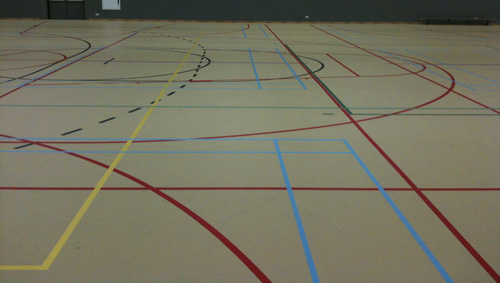
\includegraphics[width=8cm]{images/exp1-imav-floor.jpg}
\caption{Photo of the sports floor, which resambles the circumstances encountered during the IMAV competition.}
\label{fig:exp1-floor}
\end{figure}

\begin{table}[htb!]
    \centering
    \begin{tabular}
        { | l | l | l | } 
	\hline
	Method & Mean absolute error (\small{mm}) & Mean relative error (percentage of trajectory length) \\
        \hline
	AP (onboard position) & 988 & 0.960\% \\
        AV (onboard velocity) & 988 & 0.960\% \\
	AV + localization & 461 & 0.452\% \\
	VO (visual odometry) & 4251 & 4.172\% \\
	VO + localization & 1158 & 1.136\% \\
	\hline
    \end{tabular}
    \caption{Errors made by the position estimation methods when flying in circumstances encountered during the IMAV competition.}
    \label{tab:res_mapping_imav}
\end{table}

\begin{figure}[htb!]
\centering
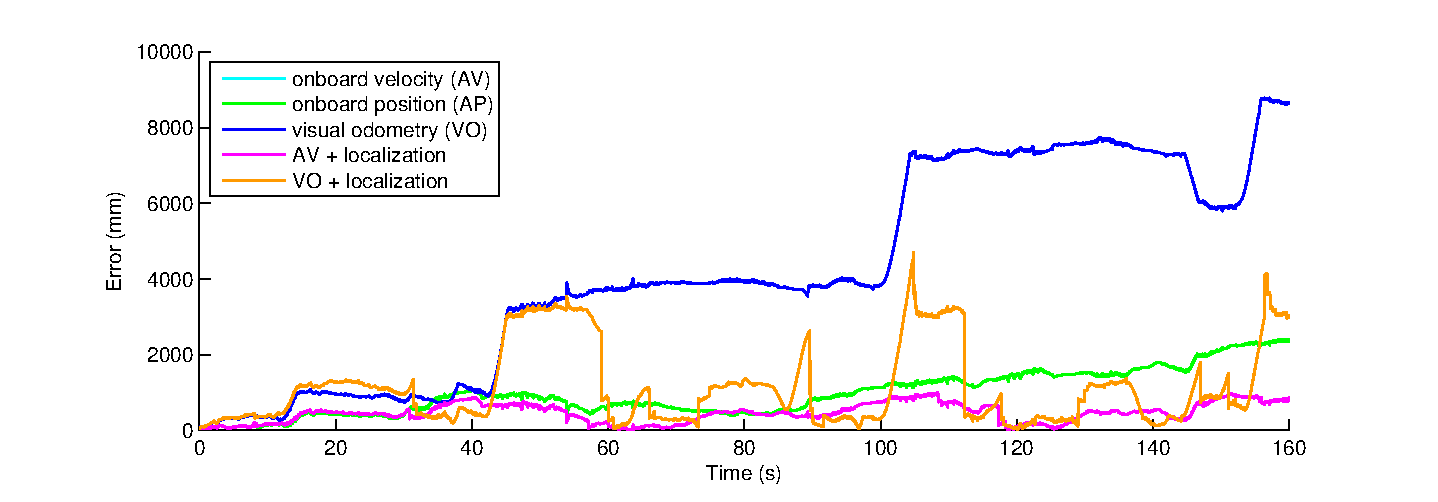
\includegraphics[width=\linewidth]{images/exp1-imav-error.eps}
\caption{Errors between the estimated positions and the groundtruth.}
\label{fig:exp1-imav-error}
\end{figure}

\begin{figure}[htb!]
\centering
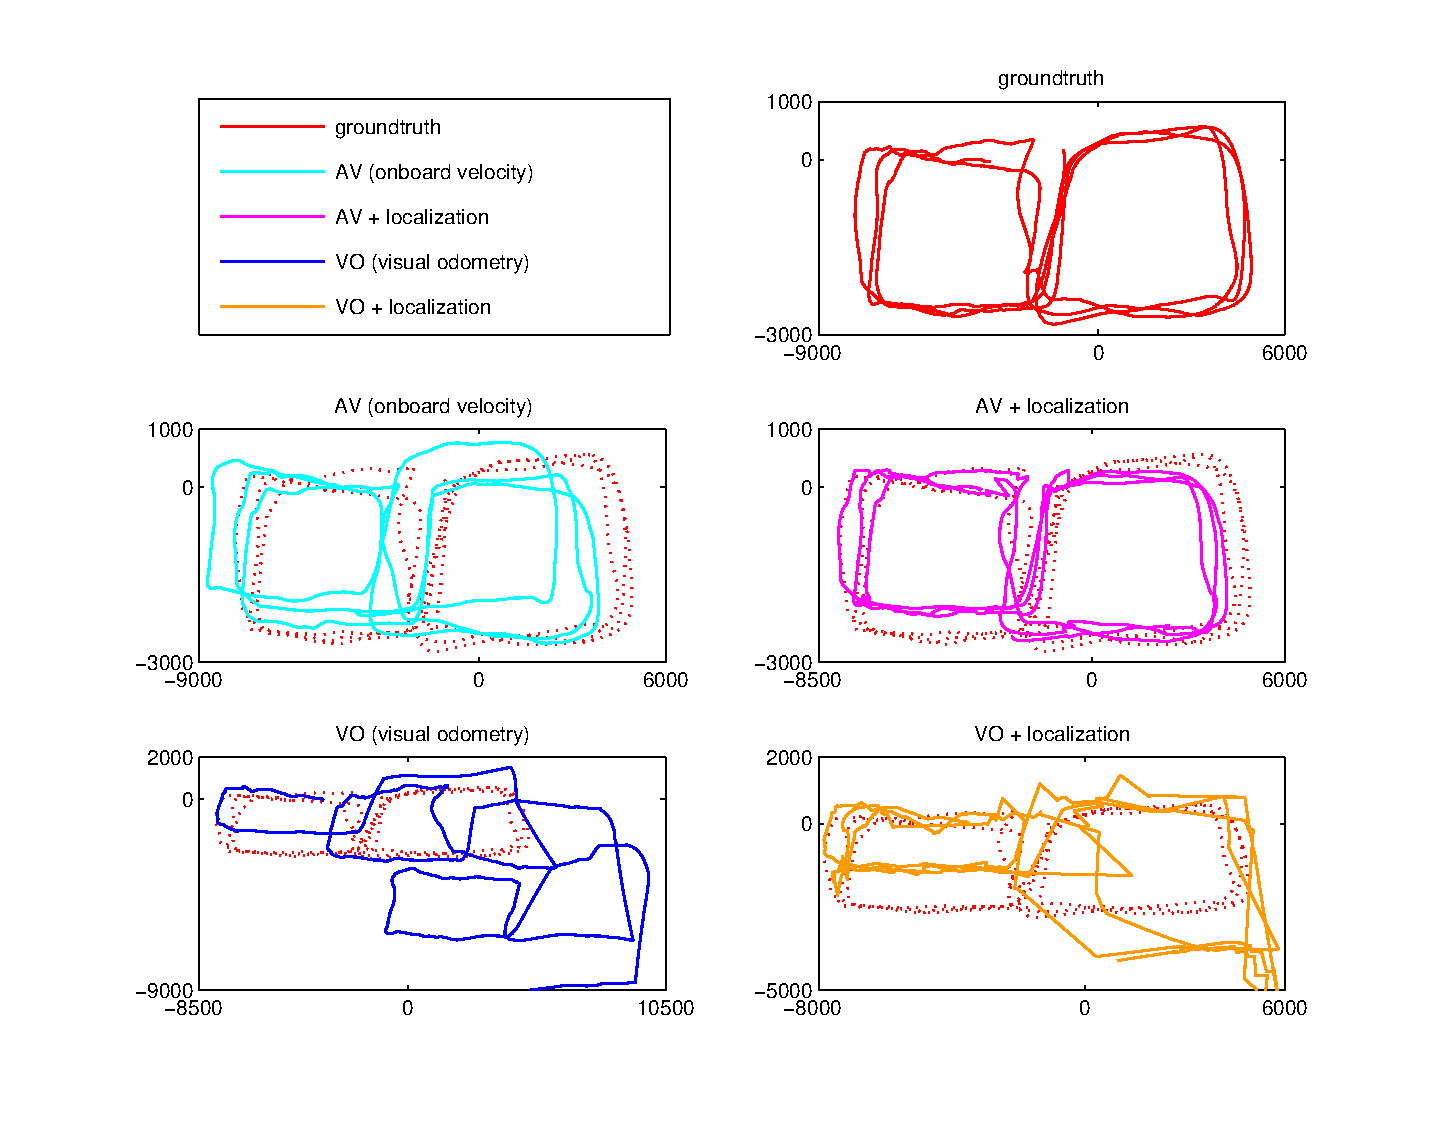
\includegraphics[width=\linewidth,trim=2cm 1.5cm 2cm 2cm]{images/exp1-imav-path.eps}
\caption{Estimated trajectories of the different position estimation methods. The AR.Drone flew three 8-shapes above a sport floor. All units are in \small{mm}.}
\label{fig:exp1-imav-path}
\end{figure}

\begin{figure}[htb!]
\centering
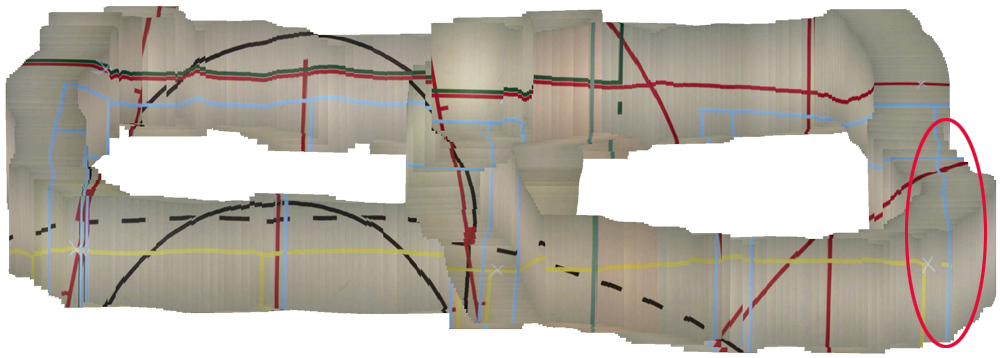
\includegraphics[width=0.75\linewidth]{images/exp1-imav-map.png}
\caption{Visual map created by the visual mapping method (Section \ref{sec:texture_map}). The map is constructed during the first 8-shape. The position estimates are based on the onboard velocity (AV) and the visual localization method (Section \ref{sec:localization}). The red ellipse indicaties an area for which the visual odometry method is unable to estimate the velocity.}
\label{fig:exp1-imav-map}
\end{figure}

The results of this experiment can be found in Table \ref{tab:res_mapping_imav} and Figures \ref{fig:exp1-imav-error} (errors), \ref{fig:exp1-imav-path} (trajectories) and \ref{fig:exp1-imav-map} (visual map).
%As noted before, both the onboard velocity (AV) method and the onboard position (AP) method produce exactly the same trajectory.
For the encountered circumstances, not all methods are able to estimate the position accurately.
The AR.Drone's onboard velocity (AV) method is able to estimate the position quite well, with an average error of $1\small{m}$.
The error increases steadily over time due to drift.
In Figure \ref{fig:exp1-imav-path} can be seen that this method underestimates the distance along the left vertical path of the trajectory.
During this path, the camera observes parallel lines, for which it is hard to recover the velocity from vision.
Similar behavior is visible for the proposed visual odometry method (VO).

%However, the error increases steadily over time due to the lack of a map.
The proposed visual odometry method (VO) is having more difficulties.
From Figure \ref{fig:exp1-imav-error} can be seen that the error of the visual odometry method (blue line) is increasing rapidly at certain moments in time.
The repetitive behavior suggests the sudden increase in error is correlated to a certain position of the floor.
Investigation showed that the visual odometry method was unable to estimate the velocity within a specific area (red ellipse in Figure \ref{fig:exp1-imav-map}).
In this area, the floor has too few visual clues.

When using localization against the map, the errors decrease significantly.
The localization method is able to recover the AR.Drone's position from the map, which reduces the drift.
However, due to the lack of a map optimization method, the map contains errors.
These errors affect the accuracy of a localization.
Therefore, a repetitive error pattern is visible.
%Because localization was possible on regular basis, the errors do not exceed the errors of the first 8-shape in which the map is build.
For each 8-shape, the errors are approximately bounded to the errors made during the first 8-shape.

These results confirm that the localization method is able to deal with circumstances encountered during the IMAV competition.
A feature-based approach to visual odometry is insufficient to estimate the velocity above all areas of a sport floor.
Therefore, an additional appearance-based method (like the AR.Drone uses) is required to estimate the velocity at all times.


\clearpage
\section{Accuracy w.r.t. pose recovery approaches}
\label{sec:results-pose-recovery}
Section \ref{sec:pose-recovery} proposed a new method to robustly recover the translation and rotation between two frames (for visual odometry) or a frame and a map (for localization).
This method features two improvements.
Instead of computing a full perspective, affine or Euclidean transformation, a more pragmatic approach is used.
Futhermore, the proposed approach uses covariance, instead of the number inliers, as quality measure.
In this experiment, the proposed pose recovery approach is benchmarked against other pose recovery approaches.
The proposed approach has been validated with the proposed covariance quality measure and with the classic \textit{inliers based} quality measure, in order to validate the contribution of the proposed quality measure.

An approach similar to the position accuracy experiment from Section \ref{sec:results-position-accuracy} is used.
The positions are estimated using the Visual Odometry (VO) method from Section \ref{sec:visual-slam-visual-odemetry}, which relies on pose recovery to determine the velocity.
The recorded dataset of the texture-rich floor (Section \ref{sec:exp1-texture-rich} ) is used as input.
 
The pose recovery approach is benchmarked against OpenCV's robust \textit{Euclidean transformation}, \textit{affine transformation} and \textit{perspective transformation}.
The \textbf{Euclidean transformation} is computed using OpenCV's \textit{estimateRigidTransform}\footnote{\url{http://opencv.itseez.com/modules/video/doc/motion_analysis_and_object_tracking.html?highlight=estimateRigidTransform}} with the parameter \textit{fullAffine} off to compute a Euclidean transformation.
The translation vector from the transformation matrix is used as velocity estimate.
The maximum allowed reprojection error is set to $10\small{mm}$.
Additional filtering is required to remove bad transformation.
A recovered transformation is rejected if the percentage of inliers is below $50\%$ or if the translation is too large ($T \geq 500\small{mm}$).
The \textbf{affine transformation} is computed using OpenCV's \textit{estimateRigidTransform}\footnote{\url{http://opencv.itseez.com/modules/video/doc/motion_analysis_and_object_tracking.html?highlight=estimateRigidTransform}} with the parameter \textit{fullAffine} on.
The \textbf{perspective transformation} is computed using OpenCV's \textit{findHomography}\footnote{\url{http://opencv.itseez.com/modules/video/doc/motion_analysis_and_object_tracking.html?highlight=findhomography}} with a RANSAC-based robust method.
The translation vector from the homography is used as velocity estimate.

\begin{table}[htb!]
    \centering
    \begin{tabular}
        { | l | l | l | } 
	\hline
	Method & Mean absolute error (\small{mm}) & \parbox{5cm}{Mean relative error \\(percentage of trajectory length)} \\
        \hline
        visual odometry (VO) & 552 & 0.828\% \\
        visual odometry (VO) - inliers based & 734 & 1.101\% \\
	visual odometry (VO) - Euclidean transform & 967 & 1.449\% \\
	visual odometry (VO) - affine transform & 3784 & 5.672\% \\
	visual odometry (VO) - perspective transform & 8923 & 13.375\% \\
	\hline
    \end{tabular}
    \caption{Errors made by the visual odometry (VO) position estimation method when using different pose recovery approaches.}
    \label{tab:res_transform}
\end{table}

The results of this experiment can be found in Table \ref{tab:res_transform} and Figure \ref{fig:exp4-transform-error}.
These results show a relation between the degrees of freedom of an approach and the errors in the estimated positions.
Reducing the degrees of freedom results in more robustness against noise.
This corresponds with the observations made by Caballero et al (Section \ref{related-online-mosaicking}).
%As explained in Section \ref{sec:pose-recovery}, classic RANSAC uses the number of inliers as quality measure.
%Because an incorrect transformation can result in a high percentage of inliers, incorrect transformations can be chosen by RANSAC.

OpenCV's pose recovery approaches use the percentage of inliers as quality measure.
However, the percentage of inliers may not reflect the actual quality of a recovered pose.
For example, a faulty transformation (pose) can maximize the number of inliers, as described in Section \ref{sec:pose-recovery}.
These faulty transformations produce sudden changes in error, as can be seen in Figure \ref{fig:exp4-transform-error}.

The proposed pose recovery approach outperforms the other pose recovery approaches.
The best performance is achieved when using the proposed convariance based quality measure.
When the confidence based quality measure is replaced with classic inliers based quality measure, the performance decreases.
However, the proposed method still outperforms the other methods.
This improvement with respect to the Euclidean transform can be dedicated to the pragmatic approach, which reduces the degrees of freedom from four (translation and rotation) to two (translation).
The additional improvement gained by the proposed approach can be dedicated to the covariance based quality measure.
This quality measure is able to estimate the quality of a recovered pose more accurately, resulting in recovered poses that contain less errors.
This is reflected by the reduced number of sudden changes in the plot.

%This approach reduces the degrees of freedom and is more robust against noise.
%The proposed approach uses the covariance between the points of a hypothesis to determine the quality of a recovered pose.
%The proposed approach uses covariance, instead of the number inliers, as quality measure.
%This approach is able to estimate the quality of a recovered pose more accurately, resulting in recovered poses that contain less errors.


\begin{figure}[htb!]
\centering
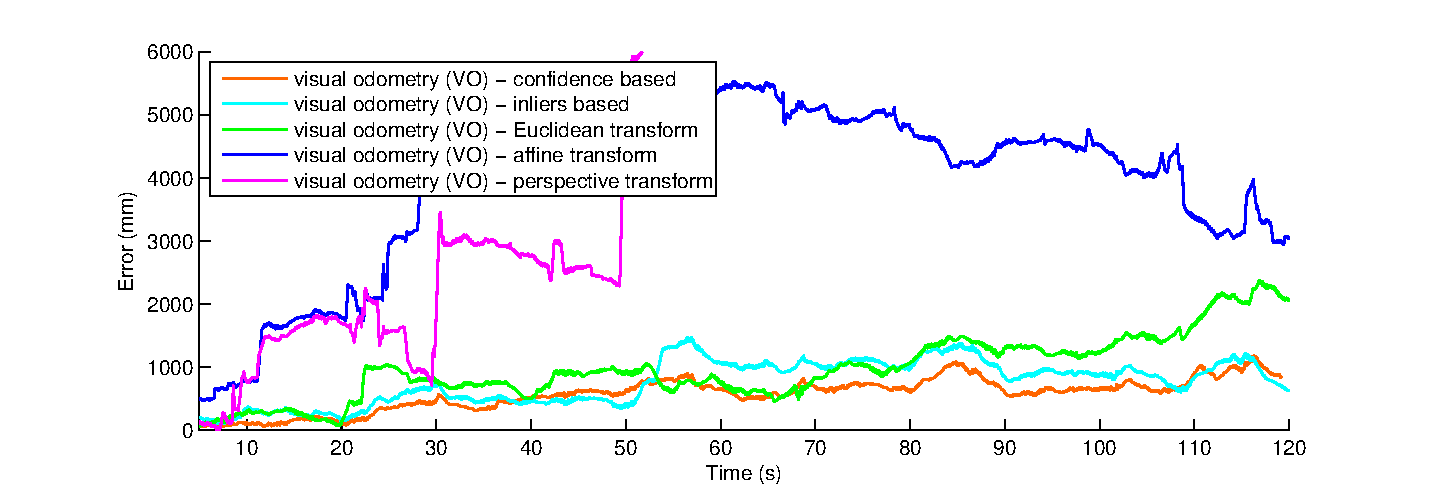
\includegraphics[width=\linewidth]{images/exp4-transform-error.eps}
\caption{Errors between the estimated positions and the groundtruth.}
\label{fig:exp4-transform-error}
\end{figure}





\clearpage
\section{Accuracy w.r.t. camera resolution}
\label{sec:res-cam-resolution}
The AR.Drone is equipped with a low resolution down-looking camera.
The recent developments in miniature high-resolution cameras enables MAVs to be equipped with high-resolution cameras.
This poses the question if the proposed method benefits from an increased image resolution.

In this experiment, the accuracy of the estimated position is evaluated for various camera resolutions.
An approach similar to the position accuracy experiment from Section \ref{sec:results-position-accuracy} is used.
The positions are estimated using the Visual Odometry (VO) method from Section \ref{sec:visual-slam-visual-odemetry}.
The recorded dataset of the texture-rich floor (Section \ref{sec:exp1-texture-rich} ) is used as input.
The experiment is repeated for different camera resolutions, which are simulated by downscaling the original camera images.
%The recorded images are downscaled to $90\%$, $66.6\%$ and $33.3\%$ of the AR.Drone's resolution.
The camera calibration matrix is scaled accordingly.

The experiment is repeated with a simulated AR.Drone in USARSim, which enables to both increase and decrease the resolution of the camera.
Attention was paid to mimic the AR.Drone's camera\footnote{A previous article \cite{Visser2011imav} describes the influence of white balancing on image stitching and how to mimic the real images as close as possible.}.

The results of the real AR.Drone can be found in Table \ref{tab:res-resolution-ar} and the results of the simulated AR.Drone can be found in Table \ref{tab:res-resolution-usar}.
For each camera resolution, the number of processed frames is counted.
Not all frames can be (accurately) related to its previous frame to determine (extract) the velocity, which is indicated by the third column.
The fourth column describes the mean error of the estimated positions.
In Figure \ref{fig:exp3-error2}, the relation between image resolution and accuracy of the estimated position is plotted.
In Figure \ref{fig:exp3-error}, the position error is plotted over time.


\begin{table}[htb!]
    \centering
    \begin{tabular}
        { | l | l | l | l | } 
	\hline
	Resolution & Nr. frames processed & Nr. frames velocity extracted & Mean error (mm) \\
        \hline
        33.3\% & 2275 & 213 & 11742 \\
	66.6\% & 2239 & 1346 & 2166 \\
	90.0\% & 2259 & 1847 & \textbf{531} \\
	100.0\% & 2168 & 1945 & 579 \\
	\hline
    \end{tabular}
    \caption{Real AR.Drone. Mean error of the estimation position for different camera resolutions. For each camera resolution, the number of processed frames is counted. A part of these frames can be used to extract the velocity of the AR.Drone.}
    \label{tab:res-resolution-ar}
\end{table}

\begin{table}[htb!]
    \centering
    \begin{tabular}
        { | l | l | l | l | } 
	\hline
	Resolution & Nr. frames processed & Nr. frames velocity extracted & Mean error (mm) \\
        \hline
        33.3\% & 1600 & 10 & 15302 \\
	66.6\% & 1580 & 266 & 601 \\
	90.0\% & 1332 & 782 & 69 \\
	100.0\% & 1383 & 1016 & \textbf{58} \\
	133.3\% & 839 & 713 & 105 \\
	166.6\% & 626 & 541 & 117 \\
	200.0\% & 407 & 398 & 128 \\
	\hline
    \end{tabular}
    \caption{Simulated AR.Drone (USARSim). Mean error of the estimation position for different camera resolutions. For each camera resolution, the number of processed frames is counted. A part of these frames can be used to extract the velocity of the AR.Drone.}
    \label{tab:res-resolution-usar}
\end{table}


\begin{figure}[htb!]
  \begin{center}
    \subfigure[Real AR.Drone]{\label{fig:exp3-2-a}%
	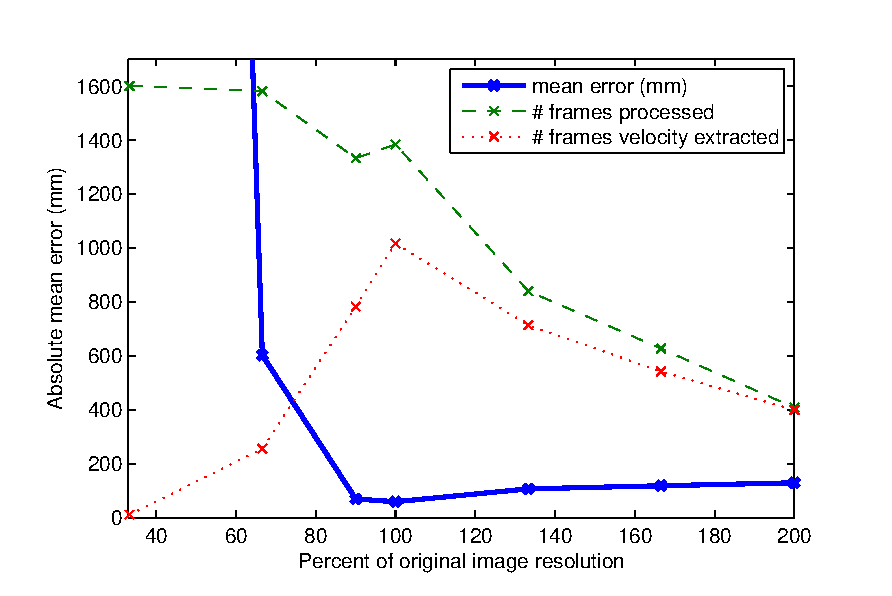
\includegraphics[width=0.55\linewidth]{images/exp3-ar-res-error2.eps}}%
    \subfigure[Simulated AR.Drone (USARSim)]{\label{fig:exp3-2-b}%
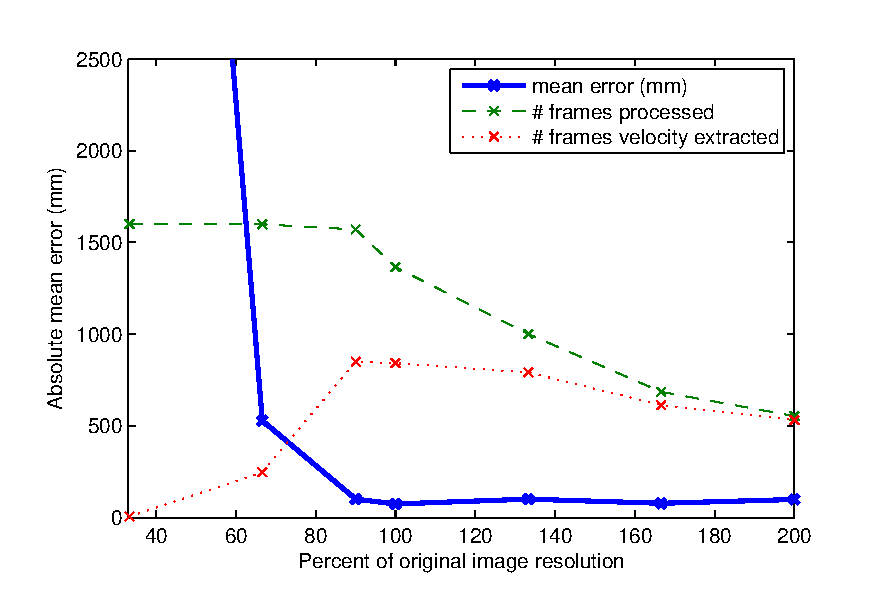
\includegraphics[width=0.55\linewidth]{images/exp3-usar-res-error2.eps}}

 \end{center}
  \caption{Mean error of the estimated position with respect to the image resolution. For each resolution, the number of processed frames is counted (green line). A part of these frames can be used to extract the velocity of the AR.Drone (red line).}
  \label{fig:exp3-error2}
\end{figure}

From Table \ref{tab:res-resolution-ar} can be seen that the original camera resolution is sufficient for frequent velocity updates.
Out of the $2168$ processed frames, $1945$ frames ($90\%$) could be used to extract the velocity using the Visual Odometry method.
When the image resolution is slightly decreased to $90\%$ of the original resolution, more frames were processed.
Algorithm such as the SURF feature extractor requires less processing time, allowing more frames to be processed.
However, only $82\%$ of these frames could be used to extract the velocity.
When the resolution decreases further, the number of processed frames remains stable, which indicates the processing time is not significantly decreasing.
However, the number of frames that could be used to extract the velocity is decreasing.
This indicates that the camera images with lower resolution are less usefull for the Visual Odometry method.
This is reflected by the mean error of the different camera resolutions.
In general, a lower camera resolution results in a larger error in the estimated position (Figure \ref{fig:exp3-2-a}).
An exception is the camera resolution of $90\%$, which has a slightly lower error than the original resolution.
This exception is probably caused by a coincidental drift that reduces the error.

The results of the simulated AR.Drone can be found in Table \ref{tab:res-resolution-usar} and Figure \ref{fig:exp3-2-b}.
The overall mean errors are smaller than the real AR.Drone, due to the lack of noise generated by the IMU and ultrasound sensor.
Similar to the real AR.Drone, a reduced resolution results in more frames being processed, but less frames that could be used to extract the velocity.
When the resolution increases, the number of processed frames decreases due to the increased computational time per frame.
However, the percentage of frames that could be used to extract the velocity increases.
This indicates that the camera images with a higher resolution are more usefull for the Visual Odometry method.
For the original resolution, $62\%$ of the processed frames could be used to extract the velocity. When the resolution is doubled, $96\%$ of the frames could be used to extract the velocity.
One would expect that an increased image resolution would result in a smaller error.
However, due to the increased computational time per frame, less frames can be processed resulting in less frequent velocity estimates.
This results in a mean error that is not smaller than the original resolution.

\begin{figure}[htb!]
  \begin{center}
    \subfigure[Real AR.Drone]{\label{fig:exp3-a}%
	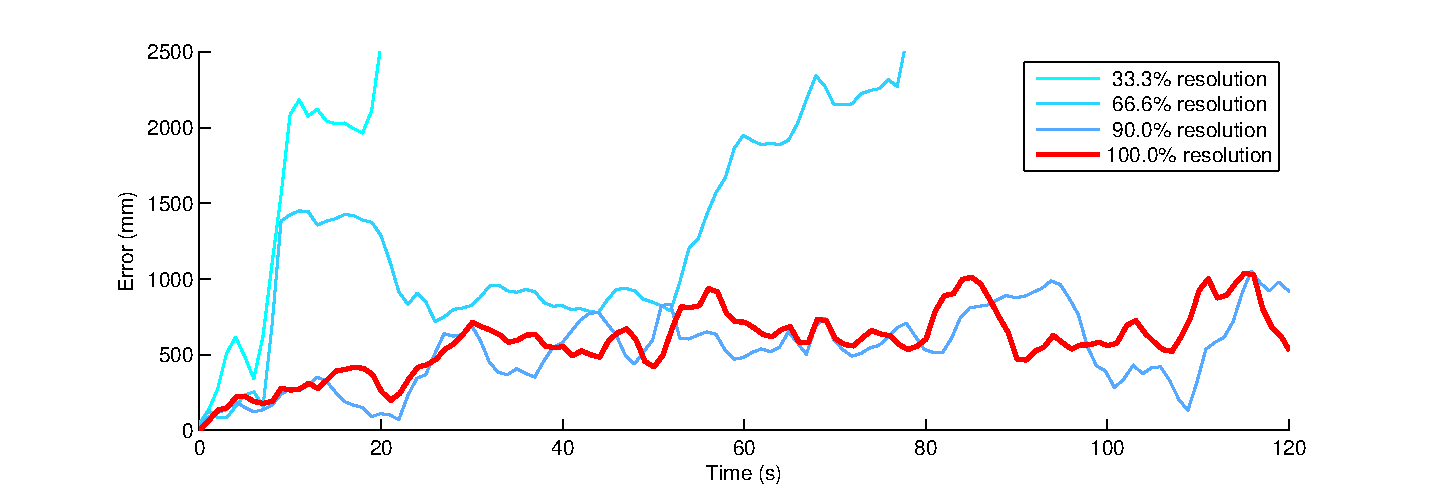
\includegraphics[width=0.9\linewidth]{images/exp3-ar-res-error.eps}}%
\\
    \subfigure[Simulated AR.Drone (USARSim)]{\label{fig:exp3-b}%
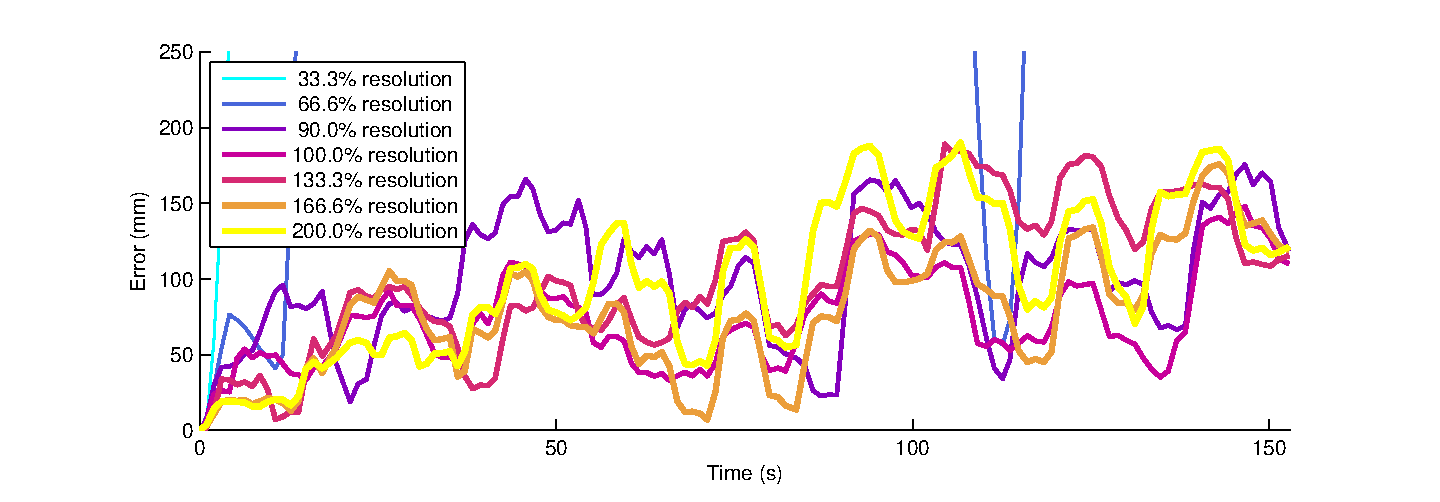
\includegraphics[width=0.9\linewidth]{images/exp3-usar-res-error.eps}}

 \end{center}
  \caption{Error of the estimated position for different image resolutions.}
  \label{fig:exp3-error}
\end{figure}




%\subsubsection{Faster computer}
\clearpage
The experiment is repeated on a faster computer\footnote{The original experiment was performed on a Intel Core 2 Duo 2.2 GHz. The experiment is repeated on a faster Intel Core i7-2600 3.4 GHz. The Passmark CPU Mark benchmark indicates a score of $1259$ vs $8891$ (higher is better). \url{http://www.cpubenchmark.net/cpu_list.php}}, to verify that an increased camera resolution is yielding improved position accuracy when velocity estimates can be computed frequently.
The results can be found in Table \ref{tab:res-resolution-usar-pcudk} and Figures \ref{fig:exp3-pcudk-res-error} and \ref{tab:res-resolution-usar-pcudk}.

For each resolution, the faster computer is able to process more frames, resulting in more frequent velocity updates.
Therefore, the mean error decreases.
Similar to the previous experiment, the number of processed frames decreases when the camera resolution increases.
This indicates that the faster computer is still unable to process all incoming frames.
The video processing implementation, which uses a single thread, is unable to make full use of the CPU's processing power.
Despite this fact, the faster computer is able to benefit from the increased image resolution.
A camera resolution of $133.3\%$ is producing the smallest mean error, outperforming the mean error from the previous experiment.
For this increased resolution, the faster computer is able to process the same amount of frames as the other computer running at the original resolution.
When the resolution increases further ($166.6\%$ or $200.0\%$), the mean error increases due to the less frequent velocity estimates.

From these observations can be concluded that the AR.Drone's bottom camera resolution offers a good balance between image quality (usefulness) and processing time.
An increased camera resolution is yielding improved position accuracy when the computer is able to process sufficient frames when the image resolution increases.
A multi-threaded implementation is expected to provide a performance boost.

\begin{table}[htb!]
    \centering
    \begin{tabular}
        { | l | l | l | l | } 
	\hline
	Resolution & Nr. frames processed & Nr. frames velocity extracted & Mean error (mm) \\
        \hline
	100.0\% & 1556 & 1145 & 69 \\
	133.3\% & 1330 & 961 & \textbf{54} \\
	166.6\% & 836 & 773 & 82 \\
	200.0\% & 655 & 624 & 83 \\
	\hline
    \end{tabular}
    \caption{(Simulated AR.Drone \& faster computer). Mean error of the estimation position for different camera resolutions. For each camera resolution, the number of processed frames is counted. A part of these frames can be used to extract the velocity of the AR.Drone.}
    \label{tab:res-resolution-usar-pcudk}
\end{table}


\begin{figure}[htb!]
\centering
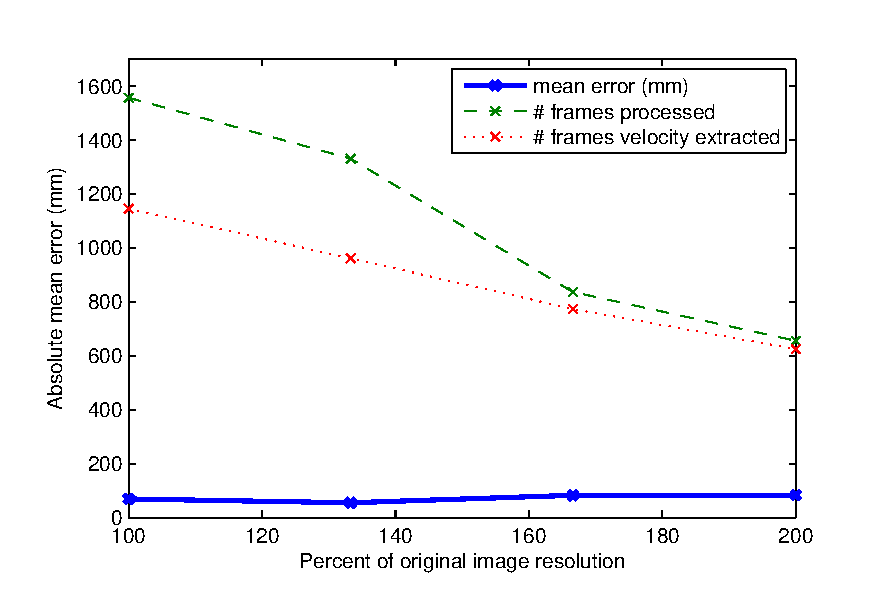
\includegraphics[width=0.55\linewidth]{images/exp3-us-pcudk2.eps}
\caption{(Simulated AR.Drone \& faster computer) Mean error of the estimated position with respect to the image resolution. For each resolution, the number of processed frames is counted (green line). A part of these frames can be used to extract the velocity of the AR.Drone (red line).}
\label{fig:exp3-pcudk-res-error}
\end{figure}

\begin{figure}[htb!]
\centering
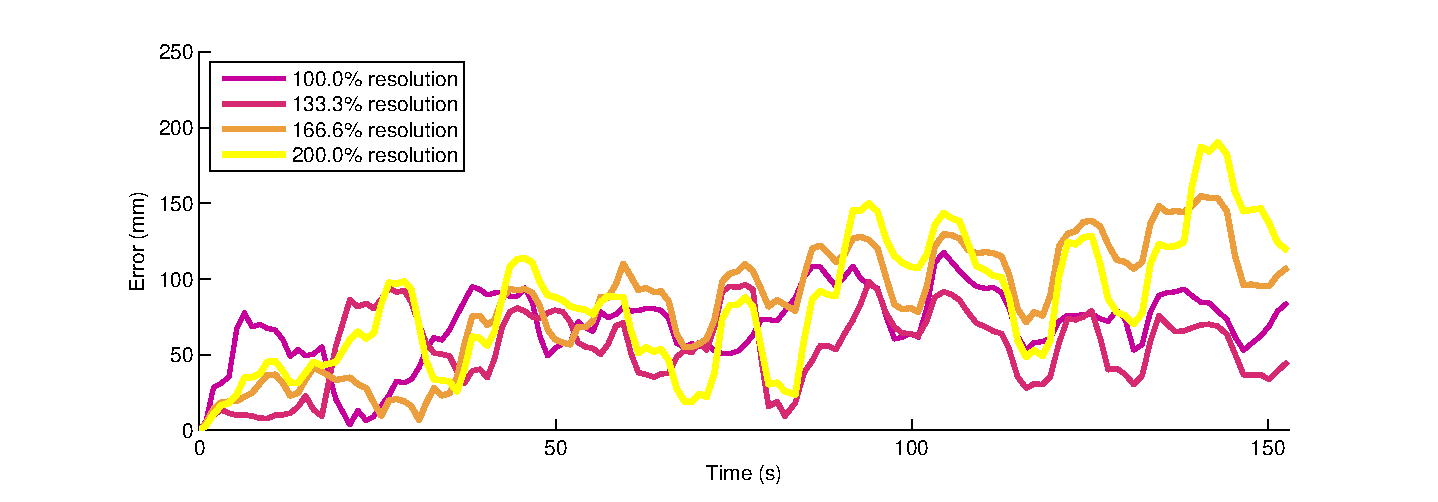
\includegraphics[width=0.9\linewidth]{images/exp3-us-pcudk.eps}
\caption{(Simulated AR.Drone \& faster computer) Error of the estimated position for different image resolutions.}
\label{fig:exp3-pcudk-res-error2}
\end{figure}







\clearpage
\section{Elevation accuracy}
\label{sec:results-elevation-accuracy}
The accurracy of the elevation map is evaluated in terms of elevation error and the error in the estimated dimensions of objects.

\subsubsection{Elevation map of a staircase}

In the first experiment, the AR.Drone flew with a constant speed over a large staircase (Figure \ref{fig:exp2-stair-photo}).
The depth of each step is $30\begin{small}cm\end{small}$ and the height of each step is $18\begin{small}cm\end{small}$.
The total height of the staircase is $480\begin{small}cm\end{small}$.
After the staircase is fully traversed by the AR.Drone, the estimated elevation is compared against the actual height of the staircase.

\begin{figure}[htb!]
\centering
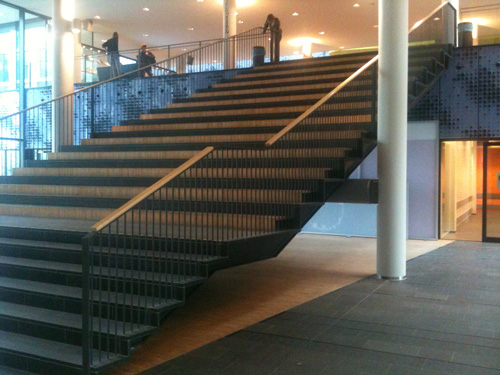
\includegraphics[width=0.4\linewidth]{images/exp2-stair-photo.jpg}
\caption{Photo of the staircase which is traversed by the AR.Drone. The depth of each step is $30\small{cm}$ and the height of each step is $18\small{cm}$. The total height of the staircase is $480\small{cm}$.}
\label{fig:exp2-stair-photo}
\end{figure}

The results of this experiment can be found in Figure \ref{fig:exp2-results}.
After fully traversing the staircase, the measured elevation is $313\begin{small}cm\end{small}$ and the error is $\frac{480 - 313}{480} \times 100 = 35\%$.
The shape of the measured elevation (Figure \ref{fig:exp2-results}) corresponds with the shape of the staircase (Figure \ref{fig:exp2-stair-photo}).
However, the approach underestimates the elevation.
When traversing the staircase, the AR.Drone's altitude stabilization increases the altitude smoothly, which causes a continuous altitude increase.
Therefore, the observed altitude difference within an elevation event is smaller than the actual altitude different caused by an object.
Another explaination of the underestimation is the error in the triggering of elevation events (due to thresholds).
When an elevation event is triggered at a suboptimal timestamp, the full altitude difference is not observed.
Ideally, an elevation UP event is triggered right before an object is detected by the ultrasound sensor, and an elevation NONE event is triggered right after the full height of the object is observed by the ultrasound sensor.


\begin{figure}[htb!]
  \begin{center}
    \subfigure[Plot of the detected elevation]{\label{fig:exp2-stair-plot}%
	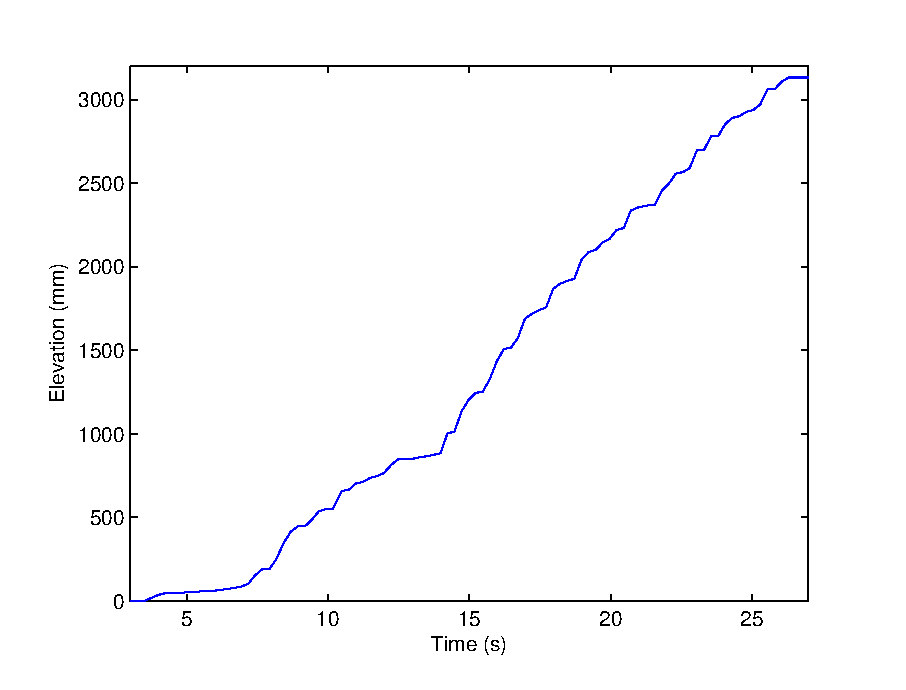
\includegraphics[width=0.55\linewidth]{images/exp2-stair-elevation-plot.eps}}%
    \subfigure[Visual elevation map]{\label{fig:exp2-stair-map}%
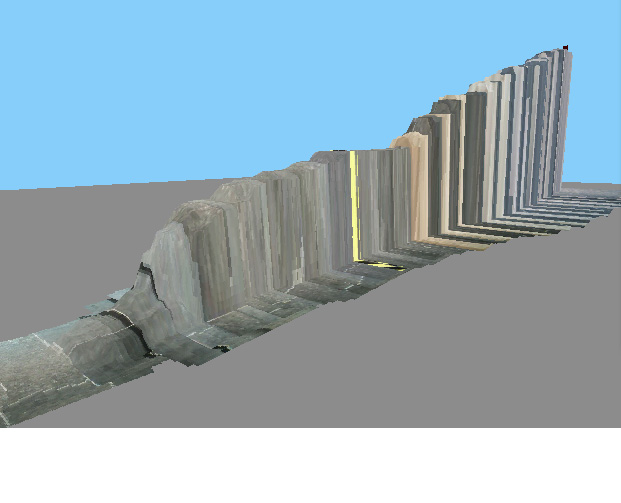
\includegraphics[width=0.4\linewidth]{images/exp2-stair-map.jpg}}

 \end{center}
  \caption{Elevation map of a large staircase (Figure \ref{fig:exp2-stair-photo}). In \ref{fig:exp2-stair-plot} the measured elevation is plotted over time. In \ref{fig:exp2-stair-map} the elevation map is rendered using the 3DTerrain component of the presented framework.}
  \label{fig:exp2-results}
\end{figure}

\subsubsection{Elevation map of multiple objects}

In the second experiment, the elevation mapping approach is evaluated in terms of error in the estimated dimensions of objects.
Objects with different dimensions were laid out on a flat floor.
A photo of the floorplan can be found in Figure \ref{fig:exp2-setup}.
The AR.Drone's trajectory, which covers all objects, is indicated with a red line.
% and the object's dimensions 
%The AR.Drone flew the marked trajectory over all objects.

\begin{figure}[htb!]
\centering
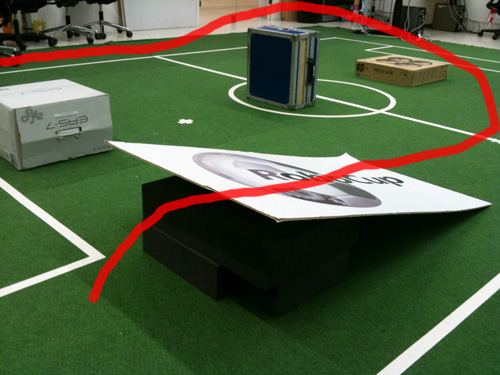
\includegraphics[width=0.4\linewidth]{images/exp2-elevation-setup.jpg}
\caption{Photo of the floorplan with different objects. The dimensions of the objects can be found in Table \ref{tab:exp2}. The red line indicates the trajectory of the AR.Drone.}
\label{fig:exp2-setup}
\end{figure}

The results of this experiment can be found in Table \ref{tab:exp2} and Figure \ref{fig:exp2-2-results}.
An object's width is evaluated in the trajectory's direction only. 
For the other direction, the width of an object cannot be estimated accurately, because the refinement step from Section \ref{sec:elevation_map} cannot be applied.


\begin{table}[htb!]
    \centering
    \begin{tabular}
        { | l | l | l | l | l | } 
	\hline
	Object & Dimensions (w$\times$h) (\small{mm}) & Estimated dimensions & Absolute error & Relative error \\
        \hline
        1. White box	& 460 $\times$ 290	& 390 $\times$ 245	& 70 $\times$ 45	& \textbf{15 $\times$ 16 \%}\\
	2. Blue box	& 245 $\times$ 490	& 250 $\times$ 420	& 5 $\times$ 70	& \textbf{2 $\times$ 14 \%}\\
	3, Brown box	& 570 $\times$ 140	& - 					& - 				& - \\
	4. Ramp		& 1380 $\times$ 360	& - 					& - 				& - \\
	\hline
    \end{tabular}
    \caption{Errors made in the estimated dimensions of objects. The first dimension is the width of an object in the y-direction and the second dimension is the height of an object. }
    \label{tab:exp2}
\end{table}

The white and blue boxes are detected.
The errors of both the estimated width and height are small.
Similar to the previous experiment, the height of an object is (slightly) underestimated.
The width of the white box is underestimated, which is probably caused by unreliable velocity estimates due to the lack of sufficient features.
Another explanation could be that the visual odometry methods assume a flat world, which does not hold when flying above objects.
Between both boxes, a false elevation is detected (clearly visible in Figure \ref{fig:exp2-elevation-plot}).
This elevation is probably triggered by a fast descent, caused by the AR.Drone's altitude stabilization, after the white box is passed.

The brown box is not detected due its limited height.
Therefore, the measured (ultrasound) acceleration is not sufficient to trigger an elevation event.
As expected, the ramp was not detected.
The gradual elevation change does not produce a significant acceleration.

\begin{figure}[htb!]
  \begin{center}
    \subfigure[Plot of the detected elevation]{\label{fig:exp2-elevation-plot}%
	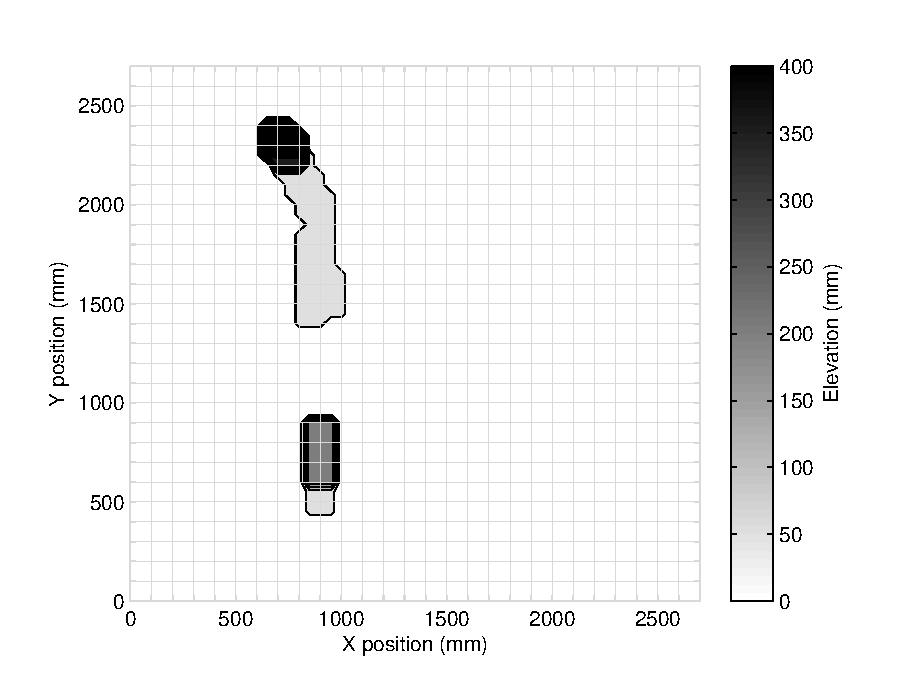
\includegraphics[width=0.55\linewidth]{images/exp2-contourf.eps}}%
    \subfigure[Visual elevation map]{\label{fig:exp2-elevation-map}%
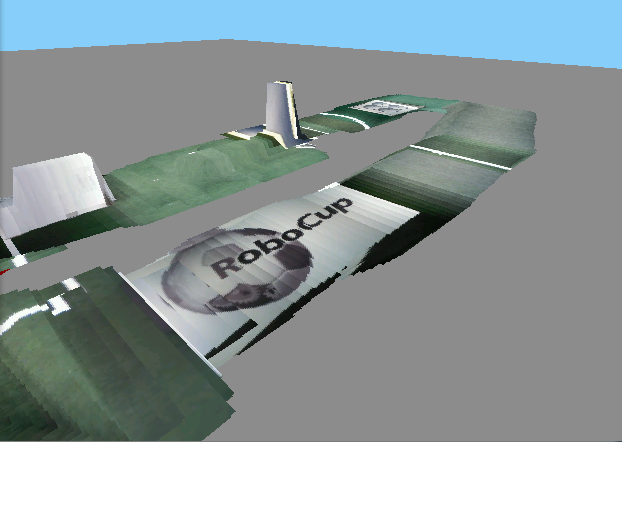
\includegraphics[width=0.4\linewidth]{images/exp2-elevation-map.png}}

 \end{center}
  \caption{Elevation map of multiple objects (Figure \ref{fig:exp2-setup}). In \ref{fig:exp2-stair-plot} a contour map of the elevation is plotted. In \ref{fig:exp2-stair-map} the elevation map is rendered using the 3DTerrain component of the presented framework.}
  \label{fig:exp2-2-results}
\end{figure}